\documentclass{beamer}
\usetheme{Frankfurt}
% \setbeameroption{show notes}
% \setbeamertemplate{note page}[plain]

\usepackage[T1]{fontenc}
\usepackage[utf8]{inputenc}
\usepackage[french,english]{babel}

\usepackage{blindtext}
\usepackage{appendixnumberbeamer}

\title{Experiments on automation of formal verification of devices at the binary level}
\subtitle{}
\author{Thomas Lacroix}
\titlegraphic{
\includegraphics[width=4cm]{logos/insa-logo-coul.png}}
\institute{INSA Lyon \\ Soutenance de PFE (Option R\&D)}
\date{19/06/2019}

% Add pages before every section and subsections
\AtBeginSection[]{\frame{\sectionpage}}
\AtBeginSubsection[]
{%
    \begin{frame}
        \frametitle{Table of Contents}
        \tableofcontents[hideothersubsections, currentsection, currentsubsection]
    \end{frame}
}

% Add page number in upper-right corner
\makeatletter
\defbeamertemplate*{headline}{my smoothbars theme}
{%
    \pgfuseshading{beamer@barshade}%
    \ifbeamer@sb@subsection%
    \vskip-9.75ex%
    \else%
    \vskip-7ex%
    \fi%
    \begin{beamercolorbox}[ignorebg,ht=2.25ex,dp=3.75ex]{section in head/foot}
    \insertnavigation{.9\paperwidth}\hfill%
    \insertframenumber/\inserttotalframenumber%
    \hspace{.5em}
    \end{beamercolorbox}%
    \ifbeamer@sb@subsection%
    \begin{beamercolorbox}[ignorebg,ht=2.125ex,dp=1.125ex,%
        leftskip=.3cm,rightskip=.3cm plus1fil]{subsection in head/foot}
        \usebeamerfont{subsection in head/foot}\insertsubsectionhead
    \end{beamercolorbox}%
    \fi%
}%
\makeatother

% To remove the navigation buttons at the bottom
% \beamertemplatenavigationsymbolsempty

% Explain NIC and what we want to prove
%   - obvious reason: connected to Internet and DMA access
%   - buffer descriptor
%       - not circular
%       - only readable memory
%       - not overlapping
%   - show that it's possible to violate the invariant
%       -> overlapping tx and rx BD
%   => need to model the spec
%   => modeled with invariants
%
% Can we reuse work done for software verification to verify hardware?
%
% Start with explanation of PP analysis vs non-PP
%
% Last 5 minutes, show every supporting tools
%   => everything that is needed that is not direct PP stuff

%%%%%%%%%%%%%%%%%%%%%%%%%%%%%%%%%%%%%%%%%%%%%%%%%%%%%%%%%%%%%%%%%%%%%%%%%%%%%%%%
%%%%%%%%%%%%%%%%%%%%%%%%%%%%%%%%%%%%%%%%%%%%%%%%%%%%%%%%%%%%%%%%%%%%%%%%%%%%%%%%
%%%%%%%%%%%%%%%%%%%%%%%%%%%%%%%%%%%%%%%%%%%%%%%%%%%%%%%%%%%%%%%%%%%%%%%%%%%%%%%%

\begin{document}

\begin{frame}
    \maketitle
\end{frame}

%%%%%%%%%%%%%%%%%%%%%%%%%%%%%%%%%%%%%%%%%%%%%%%%%%%%%%%%%%%%%%%%%%%%%%%%%%%%%%%%
%%%%%%%%%%%%%%%%%%%%%%%%%%%%%%%%%%%%%%%%%%%%%%%%%%%%%%%%%%%%%%%%%%%%%%%%%%%%%%%%
%%%%%%%%%%%%%%%%%%%%%%%%%%%%%%%%%%%%%%%%%%%%%%%%%%%%%%%%%%%%%%%%%%%%%%%%%%%%%%%%

\section{Motivation}

\subsection{Network Interface Controllers}

\begin{frame}{Security critical systems}
    \begin{columns}
        \begin{column}{0.5\textwidth}
            Privacy

            \begin{itemize}
                \item Smartphones
                \item Smart TVs
            \end{itemize}
        \end{column}
        \begin{column}{0.5\textwidth}
            Security

            \begin{itemize}
                \item Hospital equipment
                \item Traffic control systems
                \item Power plants
            \end{itemize}
        \end{column}
    \end{columns}
\end{frame}

\begin{frame}{Security critical systems - vulnerable}
    \begin{columns}
        \begin{column}{0.5\textwidth}
            https://www.wired.com/2014/04/ hospital-equipment-vulnerable/

            It's Insanely Easy to Hack Hospital Equipment
        \end{column}
        \begin{column}{0.5\textwidth}
            https://www.wired.com/2015/07/ hackers-remotely-kill-jeep-highway/

            Hackers Remotely Kill a Jeep on the Highway—With Me in It
        \end{column}
    \end{columns}
\end{frame}

\begin{frame}
    Vulnerabilities come because of:
    \begin{itemize}
        \item Increased surface of attack (more and more features, codebases explode in size)
        \item Connected to networks $\rightarrow$ remote attacks
    \end{itemize}
\end{frame}

\begin{frame}
    \begin{figure}
        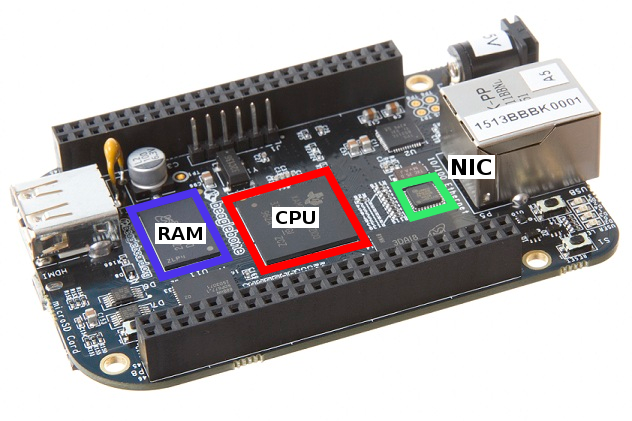
\includegraphics[]{figures/BBB_cpu_ram_nic.png}
        \caption{BeagleBone Black.}
        \label{bbb_nic}
    \end{figure}
\end{frame}

\begin{frame}
    \begin{figure}
        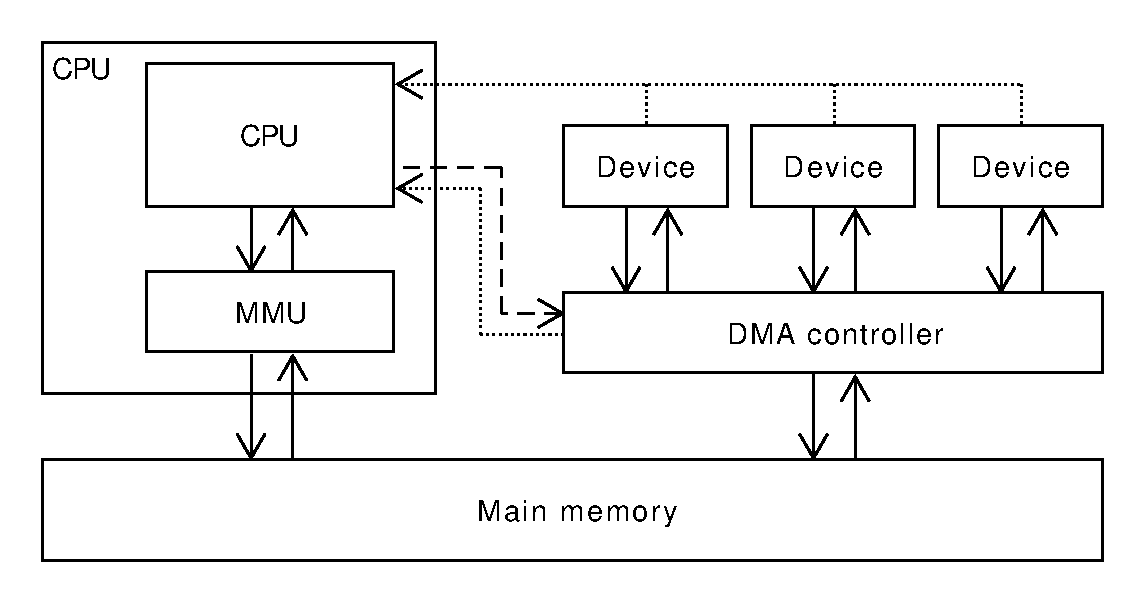
\includegraphics[width=8cm]{../figures/cpu-memory-schema.pdf}
        \caption{Communication between CPU and devices.}
        \label{cpu_mem_schema}
    \end{figure}
    \note{Dashed: register writes}
    \note{Dotted: interrupts}
\end{frame}

\subsection{How to model a NIC}

\begin{frame}{Simple frame}
\end{frame}

\subsection{Using software verification tools for hardware devices?}

\begin{frame}{Simple frame}
\end{frame}

%%%%%%%%%%%%%%%%%%%%%%%%%%%%%%%%%%%%%%%%%%%%%%%%%%%%%%%%%%%%%%%%%%%%%%%%%%%%%%%%
%%%%%%%%%%%%%%%%%%%%%%%%%%%%%%%%%%%%%%%%%%%%%%%%%%%%%%%%%%%%%%%%%%%%%%%%%%%%%%%%
%%%%%%%%%%%%%%%%%%%%%%%%%%%%%%%%%%%%%%%%%%%%%%%%%%%%%%%%%%%%%%%%%%%%%%%%%%%%%%%%

\section{Non proof-producing verification}

\subsection{Subsection 1}

\begin{frame}{Title}
\end{frame}

\subsection{How trustful is it?}

\begin{frame}{Title}
\end{frame}

\section{Proof-producing verification}

\subsection{Subsection 1}

\begin{frame}{Title}
\end{frame}

%%%%%%%%%%%%%%%%%%%%%%%%%%%%%%%%%%%%%%%%%%%%%%%%%%%%%%%%%%%%%%%%%%%%%%%%%%%%%%%%
%%%%%%%%%%%%%%%%%%%%%%%%%%%%%%%%%%%%%%%%%%%%%%%%%%%%%%%%%%%%%%%%%%%%%%%%%%%%%%%%
%%%%%%%%%%%%%%%%%%%%%%%%%%%%%%%%%%%%%%%%%%%%%%%%%%%%%%%%%%%%%%%%%%%%%%%%%%%%%%%%

\section{Conclusion}

\begin{frame}
    \begin{center}
        \huge
        Questions
    \end{center}
\end{frame}

%%%%%%%%%%%%%%%%%%%%%%%%%%%%%%%%%%%%%%%%%%%%%%%%%%%%%%%%%%%%%%%%%%%%%%%%%%%%%%%%
%%%%%%%%%%%%%%%%%%%%%%%%%%%%%%%%%%%%%%%%%%%%%%%%%%%%%%%%%%%%%%%%%%%%%%%%%%%%%%%%
%%%%%%%%%%%%%%%%%%%%%%%%%%%%%%%%%%%%%%%%%%%%%%%%%%%%%%%%%%%%%%%%%%%%%%%%%%%%%%%%

\appendix

\begin{frame}[allowframebreaks]{References}
    \bibliography{../references}
    \bibliographystyle{plain}
\end{frame}

% \begin{frame}{Backup frame}
% \end{frame}
\end{document}